\documentclass[a4paper,12pt]{article}
\usepackage[T1]{fontenc}
\usepackage{graphicx}
\usepackage{hyperref}
\graphicspath{{imagenes/}}

\begin{document}

\begin{flushleft}

\includegraphics[width=2.75cm]{unam.png}\hspace{8cm} 
\includegraphics[width=2.5cm]{fac.png}
\end{flushleft}

\begin{center}
\begin{Huge}
\texttt{UNAM}
\end{Huge}

\vspace{0.5cm}
\begin{LARGE}
\texttt{FACULTAD DE INGENIERÍA}

\vspace{0.5cm}
\texttt{INGENIERIA EN COMPUTACION}

\vspace{0.5cm}
\texttt{PROGRAMACION ORIENTADA OBJETOS}

\vspace{0.5cm}
\texttt{REPORTE GENERAL DEL PROYECTO HOTEL}

\vspace{1cm}
\end{LARGE}

\vspace{0.5cm}
\begin{LARGE}
\texttt{CARRILLO SANCHEZ RICARDO\\HERNANDEZ GOMEZ ALEJANDRO\\ZARAZUA RAMIREZ JOHAN AXEL}

\vspace{1cm}
\texttt{GRUPO: 04}

\vspace{1cm}
\texttt{PROFESOR: EDGAR TISTA GARCIA}
\end{LARGE}
\end{center}

\vspace{4cm}
\begin{flushleft}

\section{Objetivos del Proyecto}
\textsf{Se deseará aplicar los conceptos aprendidos a lo largo del curso con el fin de poder desarrollar un sistema de administración de un hotel así como aproximarse al manejo de las bases de datos con mySQL y la implementación de interfaces gráficas por medio de las clase java.swing}

\section{Introduccion}
\textsf{Para el desarrollo del sistema de administracion de un hotel nos basamos en los conceptos de la programación orientada a objetos y adicionalmente investigamos sobre conceptos básicos de bases de datos, para comenzar a modelar el sistema realizamos un esquema entidad-relacion de la base de datos ya a partir de ella se modelara el codigo, para realizar este esquema fue necesario abstraer la informacion de como funciona en la vida real un sistema de hotel y de esta forma tratar de aproximarnos a el. En este proceso se pudo identificar los diferentes campos que existen en el sistema como son trabajador, cliente, reservacion, habitaciones, pagos y servicios, y las formas en las que interactuan, es decir, como se relaciona cada uno.\\
El esquema entidad relacion que planteamos es el siguiente.}

\vspace{0.5cm}
\begin{center}
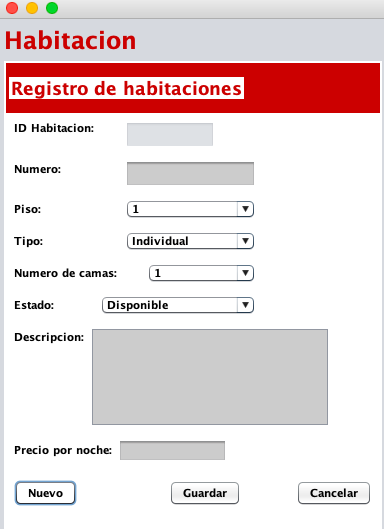
\includegraphics[width=12.75cm]{1.png}
\end{center}

\textsf{Apartir de este esquema se comenzó a codificar el sistema, separando el proyecto en tres capas la visual, logica y datos, utilizando los siguientes conceptos de P.O.O:\\}

\begin{itemize}
\item{\textbf{Bases de datos}}
\vspace{0.3cm}
\textsf{\\Una base de datos es un conjunto de datos pertenecientes a un mismo contexto y almacenados sistemáticamente para su posterior uso.\\\vspace{0.3cm}Su implementación fue en la base de datos que se realizo para modelar a los componentes del Hotel.}
\item{\textbf{Interfaces Gráficas (GUI):\\ }}
\vspace{0.3cm}
\textsf{Es un sistema de componentes visuales interactivos para software de computadora, que muestran objetos que transmiten información y representan acciones que puede realizar el usuario. Los objetos pueden cambian de color, tamaño o visibilidad cuando el usuario interactúa con ellos. Algunos de estos objetos incluyen iconos, cursores y botones. Estos elementos gráficos a veces se "mejoran" con sonidos o efectos visuales como transparencia y sombras paralelas.\\\vspace{0.3cm}Su implementación se realizo para hacer una interfaz al usuario donde este ingresará o consultará la información requerida}
\item{\textbf{Herencia y su implementación}}
\vspace{0.3cm}
\textsf{\\La herencia es el proceso que implica la creación de clases a partir de clases ya existentes, permitiendo, además, agregar más funcionalidades. Utilizando herencia la relación jerárquica queda establecida de manera implícita, partiendo de la clase más general (clase base) a la clase más específica (clase derivada). Cabe resaltar que la herencia se aplica con el fin de reutilizar código y de poder aplicar polimorfismo.\vspace{0.5cm}\\Para heredar en Java se utiliza la palabra reservada extends al momento de definir la clase, extends indicando la clase padre.\\\vspace{0.3cm}Se implementó en diversas clases para el ahorro del código, un ejemplo de estas será en la jerarquía de la clase persona y todas sus derivadas}
\item{\textbf{Polimorfismo}}
\vspace{0.3cm}
\textsf{\\El polimorfismo consiste en conseguir que un objeto de una clase se comporte como un objeto de cualquiera de sus subclases. Se puede aplicar tanto a métodos como a tipos de datos. Clasificándose en dinámico o estático\\\vspace{0.3cm}Se implementa de manera específica en las clases del paquete lógico donde el método insertar realizara Polimorfismo según del objeto que se este tratando}
\item{\textbf{Manejo de interfaces y de clases abstractas}}
\vspace{0.3cm}
\textsf{\\Podemos definir a las clases abstractas como aquellas clases que por sí mismas no se pueden identificar con algo 'concreto', pero poseen determinadas características que son comunes en otras clases que pueden ser creadas a partir de ellas.\\\vspace{0.3cm} Por otro lado podemos definir a las interfaces como la definición de un medio común en el cual se establecerán comunicaciones entre objetos que se hayan implementado dicha interfaz\\\vspace{0.3cm}Para el caso de las clases abstractas se definió C como la clase base para las clases que componen al paquete logico, siendo esta la superclase. Por otro lado, se creó una interfaz VentanaRegistros en la cual se establecen las acciones mas en comunes de las interfaces gráficas}
\item{\textbf{Manejo de excepciones}}
\vspace{0.3cm}
\textsf{\\El termino excepción hace referencia a las situaciones extraordinarias en las cuales se ve interrumpido el flujo normal de un programa durante su ejecución. La excepciones se clasifican es dos, verificadas y no verificadas. Las excepciones que se trabajaron en el desarrollo de nuestro programa son las excepciones verificadas, las cuales se caracterizan por aparecer en el tiempo de ejecución, y en el caso particular de Java estas excepciones son hijas de la clase RunTimeException o de alguna de sus subclases. \\\vspace{0.3cm}Para manejar una excepción se utilizan las palabras reservadas try y catch. El bloque try es utilizado para definir el bloque de código en el cual una excepción pueda ocurrir. El o
los bloques catch son utilizados para definir un bloque de código que maneje la excepción. Las excepciones son objetos que contienen información del error que se ha producido. Heredan de la clase Exception que a su vez hereda de la clase Throwable.\\\vspace{0.3cm}El código esta lleno de estas, desde para la implementación de los hilos para establecer la relación entre GUI's, tanto el manejo de las excepciones para el control de que el usuario ingrese datos erroneos\\\vspace{0.3cm}}
\item{\textbf{Clases envolventes}}
\vspace{0.3cm}
\textsf{\\Una clase envolvente da la funcionalidad de una clase para un tipo de datos primitivo. Estas clases envolventes tienen métodos que permiten manipular el tipo de dato primitivo correspondiente que ellos envuelven. Las clases envolventes se deben utilizar cuando  se quiere proveer de algunas funciones utilitarias para un tipo de dato en particular\\\vspace{0.3cm}Existe algunos atributos de la clase datos que están definidos como String o Int, sin embargo al momento de capturar los datos en la interfaz gráfica muchas veces estos se manejan como otro tipo, asi que para su conversión a otro tipo, se utilizan los wrappers.}
\item{\textbf{Modificadores de acceso}}
\vspace{0.3cm}
\textsf{\\Los modificadores de acceso permiten dar un nivel de seguridad mayor, restringiendo el acceso a diferentes atributos, métodos, constructores asegurándonos que el usuario deba seguir una "ruta" especificada por nosotros para acceder a la información.}
\item{\textbf{Métodos de clase}}
\vspace{0.3cm}
\textsf{\\Un método de instancia es el que se invoca siempre sobre una instancia (objeto).}
\item{\textbf{Manejo de archivos}}
\vspace{0.3cm}
\textsf{\\Un archivo es un objeto en una computadora que puede almacenar información, configuraciones o comandos, el cual puede ser manipulado como una entidad por el sistema operativo o por cualquier programa o aplicación. \\\vspace{0.3cm}Para poder manejar archivos será necesario entender el concepto de flujo, el cual lo podemos definir como una conexión entre el programa y la fuente (lectura) o el destino (escritura) de los datos. La información se traslada en serie a través de esta conexión. El flujo se puede ver como de caracteres o bytes, y dependiendo de esa perspectiva existen diferentes clases para poder manejar diferentes tipos de archivos\\vspace{0.3cm}Se realizó un diseño de facturas para el cliente, en el cual se crea un archivo del tipo PDF al momento en que este genera su pago por la habitación.}
\item{\textbf{Implementación de un patrón de diseño (Singleton)}}
\vspace{0.3cm}
\textsf{\\Es un patrón de diseño que se caracteriza por garantizar que una clase solo tenga una instancia y proporcionar un punto de acceso global a ella.\\\vspace{0.3cm}Se definio una instancia Singleton en el momento en el que se realiza la conexión con la base de datos, esta intancia se definió con el tipo "eager", con el fin de no crear mas instancias al momento de conectarse a la Base de Datos}
\end{itemize}

\textsf{\\Gracias a los conceptos previos y mas en especifico a las investigaciones que se llevaron a cabo sobre base de datos podemos hacer que en una tabla tengamos un columna  con la cual podamos ligar columnas de otra tabla, esto lo hicimos ya que detectamos que en el sistema podríamos tener una composición de objetos ya que una reservación tiene un cliente, un trabajador, una habitación, etc. Por lo tanto pudimos hacer estas composición  a partir de la base datos haciendo que no exista una composición de clases en el código de Java y favoreciendo a una cohesión baja. En conclusión podemos decir que las relaciones entre las tablas de la base de datos son muy importantes para el diseño de nuestro problema ya que a partir de ellas podemos hacer que ciertos datos tengan una conexión pero sin depender de otros, por lo que podemos eliminar  sin tanto problema ya que estaremos seguros de que solo se elimina el dato que nos interesa y no otros datos, esto lo podemos ver en la relación de pagos y reservación ya que podemos eliminar un pago sin eliminar una reservación, en cambio si esto se realiza por composición de objetos podría darse el caso de que al eliminar un pago también eliminemos una reservación,  si esto lo vemos en un aspecto Real podría suceder que un trabajador se equivoque al registrar un pago y al eliminarlo, eliminaría con el a la reservación por lo que tendrías que volver a crear la reservación y posteriormente crear de nuevo el pago.}

\section{Conclusiones:}

\begin{itemize}
\item{\textbf{Carrillo Sanchez Ricardo}}
\vspace{0.3cm}
\textsf{\\Los objetivos planteados se cumplieron con éxito, sin embargo, el desarrollo de nuestro software fue excesivamente tardado y con muchos contratiempos ya que en los componentes que nosotros le abordamos no teníamos un dominio y en algunos casos carecíamos de noción. Algunos de los contratiempos y dificultades que se nos presentaron para el desarrollo de nuestro software fue la interacción entre las interfaces gráficas, ademas de su desarrollo; personalmente yo encontré muy arduo el diseño de una interfaz gráfica ya que cometía el error de copiar elementos de algunas de las interfaces previas de las cuales ya habíamos diseñado y debido a ello en diversas ocaciones se perdía noción del identificador de estos componentes de la interfaz gráfica, curiosamente encontré el manejo de la base de datos muy practico ya que nos ahorro mucho código, tomando en cuenta que nuestro entorno de desarrollo hacia gran parte del código, y eso fue de mucha ayuda pero a su vez perjudicial ya que había ocaciones en la cuales no teníamos mucha idea de lo que hacia ese segmento de código creado por nuestro IDE, por que nos teníamos que detener a investigar. Por otro lado hubo un poco de ambigüedad de como se iban a utilizar los archivos en nuestro proyecto ya que la idea era de que el sistema proporcionara una factura al cliente en formato de pdf, y aunq que su implementación de esto no fue del todo difícil, si requirió de un análisis extra por parte del equipo.\vspace{0.3cm}\\Personalmente he encontrado el proyecto bastante remunerador, ya que se aplicaron casi en su totalidad todos los conceptos vistos e implementados en el curso ademas de que se transcendió por medio de la base de datos y la GUI. A pesar de que nos separamos un poco de los requerimientos de lo que se solicitaba, creo que nuestro desarrollo cumple con los requisitos planteados.}

\item{\textbf{Hernández Gómez Alejandro}}
\vspace{0.3cm}
\textsf{\\En definitiva el objetivo propuesto por nuestra parte se cumplió en su totalidad, en conjunto fuimos capaces de aplicar los conocimientos generales del curso en una sola aplicación o programa. Desde los aspectos básicos hasta adicionales del paradigma sirvieron para construir un código en el cual plasmamos, con ayuda de un análisis previo, la idea de un sistema administrativo de hoteles.\vspace{0.3cm}\\La parte teórica y práctica de la materia, al igual que información consultada por internet, nos facilitaron varios procesos del código, siendo un pilar fundamental en la planeación de cada paso. Creo que el extender el proyecto con ayuda de la base de datos fue de suma importancia, ya que el aprendizaje sobre este tema juega un rol importante para futuras aplicaciones, incluso va dirigido como un complemento para la planificación de clases y sus relaciones.\vspace{0.3cm}\\A parte de lo mencionado, considero que ver algo nuevo siempre es interesante en lugar de repetir procesos ya aplicados. Sin más, supongo que es todo, las dificultades que surgieron durante la realización del proyecto fueron escasas, la base contribuyó a disminuir de gran manera el número de errores que uno podría generar y el uso de interfaces ahorró de manera interna varias tareas en cuanto a la relación.}

\item{\textbf{Zarazúa Ramirez Johan Axel}}
\vspace{0.3cm}
\textsf{\\Para mi el proyecto final cumplió satisfactoriamente con los objetivos, tanto generales como particulares ya que durante su planeación e implementación se pusieron en práctica muchos de los conceptos vistos durante el curso y se aprendió un poco sobre bases de datos. En particular a mi me pareció un proyecto bueno gracias a los objetivos particulares del equipo, el incluir una base de datos nos representó un reto ya que ninguno de los integrantes tenía un conocimiento amplio sobre el tema, por lo cual tuvimos que investigar comandos, relaciones entre tablas y muchos otros temas que nos aporta un conocimiento básico pero útil para futuras materia, sin embargo debido a el poco conocimiento se nos presentaron diversos problemas durante el desarrollo del sistema, de los cuales no teníamos una idea clara de cómo resolver y tampoco se encontraba una ejemplo de cómo hacerlo, este tipo de errores, para mi, son los que forjan a un programador ya que tuvimos que deternos un poco analizar la situación, pensar en donde podría estar el error y como solucionarlo. En conjunto estos error, el repaso de conceptos y los nuevos aprendizajes convirtieron un proyecto que en un inicio pensé que sería algo un poco aburrido y repetitivo, en un proyecto muy completo}

\end{itemize}
\end{flushleft}
\end{document}